

\section{Conceptual framework} \label{sec:cf}

%% Suppose the firm has a collection of tasks that want performed which they can order for most to least valuable.
%% Let $v(L)$ be the marginal value of the task completed when $L$ efficiency units of labor are applied to the project.
%% If the firm hires a worker with productivity $y$ who works $h$ hours, $L = hy$.
%% The firm's decision of how many hours to buy is
%% \begin{align}
%%   \arg\max_{h^*} \quad \int_0^{h^*} v(hy) dh - wh^{*}  
%% \end{align} 
%% where $w$ is the worker's wage.
%% The firm's first order condition is simply $v(h^*y) = w$, i.e., where the value of output from the marginal hour is the wage.
%% This implies that $\epsilon^h_y = -1$, or that hiring a more productive worker simply means that fewer hours are purchased, even at the same price.
%% Suppose that worker offers a value multiplier on $e^{q_i}$.
%% The first order condition is now
%% \begin{align}
%%   e^{q} v(h y) = w.
%% \end{align} 
%% We have
%% \begin{align}
%%   h'(q) = - \frac{v(hy)}{y v'(hy)}
%% \end{align} 
%% \begin{align}
%%   \frac{h'(q)}{h(q)} = - \frac{v(hy)}{hy v'(hy)} > 0. 
%% \end{align}
%% \begin{align}
%%   q \frac{h'(q)}{h(q)} = - q \frac{1}{\epsilon^v_L}.
%% \end{align}



%% Suppose a firm has a project of size $Y$, which it can sell in the product market for $pY$.
%% If you hire a more productive worker, hours-worked goes down.
%% If you hire a worker with more surplus, the
%% Suppose the firm hires a worker with productivity technical productivity $y$, but who has latent quality effect $e^q$.
%% The firm's payoff is $pYe^{q_i} - w_i \frac{Y}{y}$.


The equilibrium in matching markets is profoundly shaped by search costs \citep{rogerson2005search}.
Much of these search costs are incurred by learning about the attributes of the other side of the market.
For example, job-seekers must learn about the existence of job openings, their individual probability of being hired, and at what wage.
Firms have to learn about the productivity and preferences of individual applicants. 
Some of the information needed in this match-making is provided willingly and credibly by market participants.
In particular, ``horizontal'' information such as the kind of work that is to be done, the location, the name of the firm and so on is typically provided truthfully.
Although this information is cheap talk, it works to coordinate the two sides and firms and workers have no strategic incentive to mislead \citep{farrell1996cheap}.
Other kinds of information such as educational background, criminal record or employment history are generally reported truthfully, even though a believed lie could be helpful, as third parties stand ready to verify that information \citep{autor2008economics}. 

Other kinds of information are important, but would not be viewed as credible if simply stated, and so they are signaled \citep{spence1973job}.  
In the classic case of education in the labor market, only high ability workers would choose to get costly education, and so a firm views education as a signal of ability.
In this case, the supply side of the market is vertically differentiated and the high-types want a separating equilibrium in which they are paid for their true productivity. 
Although it is the case that all else equal, the firm would prefer a more productive worker over a less productive worker at the same price, as in product markets, firms have vertical preferences.

Several recent papers have considered the effect of signaling in matching markets, in settings different to ours.
For example, \cite{lee2011propose} and \cite{coles2013preference} both consider the introduction of market interventions that make it easier for one side of the market to signal the other (participants in dating markets in the former, applicants in the academic job market in the latter).
In this case the signaling is a matter of horizontal differentiation.
By contrast, our paper focuses on signaling preferences over a vertically differentiated dimension, which brings with it the attendant risks of price markups and adverse selection as noted above.  

Most closely related to our paper is \cite{tadelis2011information}, who consider information disclosure in the wholesale auction market for used cars.
However, the signal is sent by the platform about the attributes of a good;
our signal is sent by the buyer about their preferences. 
In their experimental setting, information about used cars is {\em exogenously} randomly disclosed to market participants, before they choose which use car auctions to join.
This information disclosure induces a sorting effect that increases competition among similar-minded bidders for each type of car, and increases expected revenues---most strongly for cars at the extremes of the quality spectrum.

There are two major differences in our setting from \cite{tadelis2011information}.
First, in many markets honest information disclosure cannot be compelled (not least because the market operator may not possess the means or information to ensure it).
We focus on a setting where employers must {\em endogenously} choose whether or not to honestly signal workers about their preferences, and we find honest disclosure as a strong empirical result.
Second, the results of \cite{tadelis2011information} suggest that we should uniformly see {\em lower} wage bids in the sorted marketplace; however, we see wage markups in high tier jobs. 
As noted above, this is because the relative balance of demand and supply in the marketplace shifts bargaining power in the high tier from employers to workers. 

\cite{tadelis2011information}

\cite{anand2011} explores the role of advertising in communicating product attribtues to consumers. 
The context is television advertising for other television programs.
The authors fit a structural model, and find that exposure to a single advertisement reduces the probability of that viewer viewing their best option. 

Competitive information disclosure.
\cite{board2015competitive}

\cite{board2009}

\cite{budish2011}
\cite{cho2014}
\cite{day1976}
\cite{Silva2008}
\cite{Diamond1991}
\cite{Genesove1993}
\cite{gilson1984}
\cite{grossman1981}
\cite{healy2001}
\cite{jin2003}
\cite{johnson2006}
\cite{levin1996}
\cite{lewis2011}
\cite{milgrom1981}
\cite{Milgrom1982}
\cite{overby2009}
\cite{porter1995}
\cite{roberts2014}

\cite{coles2009signaling}
\cite{lee2009interviewing}
\cite{ely2009hiring}
\cite{ely2013adverse}
\cite{lee2011propose}
\cite{kushnir2013harmful}


Much of these search costs are incurred by learning about the attributes of the other side of the market.
For example, job-seekers must learn about the existence of job openings, their individual probability of being hired, and at what wage.
Firms have to learn about the productivity and preferences of individual applicants. 
Some of the information needed in this match-making is provided willingly and credibly by market participants.
In particular, ``horizontal'' information such as the kind of work that is to be done, the location, the name of the firm and so on is typically provided truthfully.
Although this information is cheap talk, it works to coordinate the two sides and firms and workers have no strategic incentive to mislead \citep{farrell1996cheap}.
Other kinds of information such as educational background, criminal record or employment history are generally reported truthfully, even though a believed lie could be helpful, as third parties stand ready to verify that information \citep{autor2008economics}. 

Other kinds of information are important, but would not be viewed as credible if simply stated, and so they are signaled \citep{spence1973job}.  
In the classic case of education in the labor market, only high ability workers would choose to get costly education, and so a firm views education as a signal of ability.
In this case, the supply side of the market is vertically differentiated and the high-type workers want a separating equilibrium in which they are paid for their true productivity. 
Although it is the case that all else equal, the firm would prefer a more productive worker over a less productive worker at the same price, as in product markets, firms have vertical preferences.

\cite{che2016} considers the college admissions process, showing the decentralized equilibrium has a number of flaws.

In the \cite{coles2013preference} case, preferences are over the other side of the market.
Signals essentially serve to overcome a coordination failure. 

By contrast, our paper focuses on signaling preferences over a vertically differentiated dimension, which brings with it the attendant risks of price markups and adverse selection as noted above.  


\cite{tadelis2011information}
\cite{Genesove1993} for an exploration of adverse selection in the used car market. 

\cite{anand2011} explores the role of advertising in communicating product attributes to consumers. 
The context is television advertising for other television programs.
The authors fit a structural model, and find that exposure to a single advertisement reduces the probability of that viewer viewing their best option. 


Competitive information disclosure.
\cite{board2015competitive} present a model where sellers decide how much to reveal about a product when sellers must engage in costly search.
They should that disclosure policy depends on the seller's beliefs about buyers. 

A literature that is largely theoretical. 
% \cite{board2009}---seems to auction-specific. 

\cite{budish2011}
\cite{cho2014}
\cite{day1976}
\cite{Silva2008}

In an influential theory paper, \cite{Diamond1991} show that revealing public information can reduce a firm's cost of capital by making their securities more liquid, which in turn attracts more large investors. 


\cite{gilson1984}
\cite{grossman1981}
\cite{healy2001}

Traditionally, making information public and salient exogenously has been a tool of public policy. For example, \cite{jin2003} shows that the introduction of hygiene quality report cards had a number of salutary effects, including higher scores and reduced food-related illness.
In designed markets, information disclosures can be the market designer.
But these are not free---someone has to generate the information.
In contrast, endogenous signals are cheap. 

\cite{johnson2006}
\cite{levin1996}

Despite the obvious possibility of adverse selection, many markets that would seem to be prone to adverse selection seem to work well in practice, in party by contracting on quality.
\cite{lewis2011} shows that on eBay, the revelation of information about quality (through descriptions and prices) and the contracts created by these disclosures overcome the adverse selection problem.
Our situation is not about object quality, but about the preference of a seller.
This is obviously not subject to contract. 

\cite{milgrom1981}
\cite{Milgrom1982}
\cite{overby2009}
\cite{porter1995}
\cite{roberts2014}
%\cite{coles2009signaling}
\cite{lee2009interviewing}
%\cite{ely2009hiring}

\cite{ely2013adverse}is a model of firms interviewing in a multi-stage market, where interview decisions can lead to adverse selection, with all but the highest-ranked firms excluded from the market. 


\cite{lee2011propose}
\cite{kushnir2013harmful} shows that this kind of preference signaling is not necessarily beneficial, in that it can reduce the total number of matches. 


\subsection{A simple signaling model}
If a firm hires a worker with productivity $y$ at a wage $w$, the firm gets a pay-off of $vy - w$, where $v > 0$ is the value the firm places on the output and is intended to capture the firm's vertical preferences.
There are two kinds of firms, in equal proportion: those that value a unit of productivity at $v = 1$, and those that value it at $v = v_L < 1$.
Note that our first research question, (\ref{q1}), is about whether this assumed heterogeneity exists, i.e., whether firms are meaningfully differentiated on this vertical dimension.

There are two kinds of workers: high types with productivity $y = 1$, and low-types with still-positive productivity $y = y_L < 1$.
The two worker-types also exist in equal proportion. 
Firms and workers bargain over the surplus generated, with each side getting half of the surplus. 

\paragraph{Paired at random}
To start, workers and firms are paired at random.
Both worker types and firm types are private information, ex ante.
As such, the two sides split the expected surplus, and so high- and low-type firms get 
\begin{align} \label{eq:pooling}
  \pi_H  = \mathbb{E}[y] - \frac{1}{2}\mathbb{E}[y]\mathbb{E}[v] \quad \mbox{and} \quad \pi_L  = v_L \mathbb{E}[y] - \frac{1}{2}\mathbb{E}[y]\mathbb{E}[v], \nonumber
\end{align}
respectively. 
Both firms have to pay the same wages, and the the high type firms are better off. 

\paragraph{Binary signal - no sorting}
Now consider that firms can send a binary signal, $s \in \{0,1\}$.
Consider a scenario in which all high-type firms send $s = 1$ and all low-type firms send $s = 0$.
Assume that workers do not sort but instead just apply to whatever opening they would have in the absence of the signal.
This lack of sorting is common knowledge.
Firms get paired with the same workers they would have before, but those workers know what kind of firm they face, and so the bargaining outcome changes.
The new firm payoffs are 
\begin{align}
  \pi_H = \mathbb{E}[y] - \frac{1}{2}\mathbb{E}[y] \quad \mbox{and} \quad \pi_L = v_L \mathbb{E}[y] - \frac{1}{2}\mathbb{E}[y]v_L. \nonumber 
\end{align} 
Note that high-type firms are strictly worse-off compared to the situation in Equation~\ref{eq:pooling}. 
The problem for high-type firms is that they do not get better workers, but rather just see their wage bill rise, as the workers know they firm is getting more surplus from the same expected output.
For the same reason, the low-type firms are better off because their wage bill falls.
The conjecture that workers will condition their bids on the employer's type is research question \ref{q5}.
If workers will not sort but do condition on the firm's preferences, we would not anticipate a separating equilibrium, and so the answer to our research question, (\ref{q2}), would be that firms knowing their preferences will be revealed to workers will choose to pool.   

\begin{figure} 
\caption{Possible equilibria depending on the productivity of low-type workers and the valuation of low-type firms \label{fig:illustrate_equilibria}} 
\centering 
\begin{minipage}{0.80 \linewidth}
 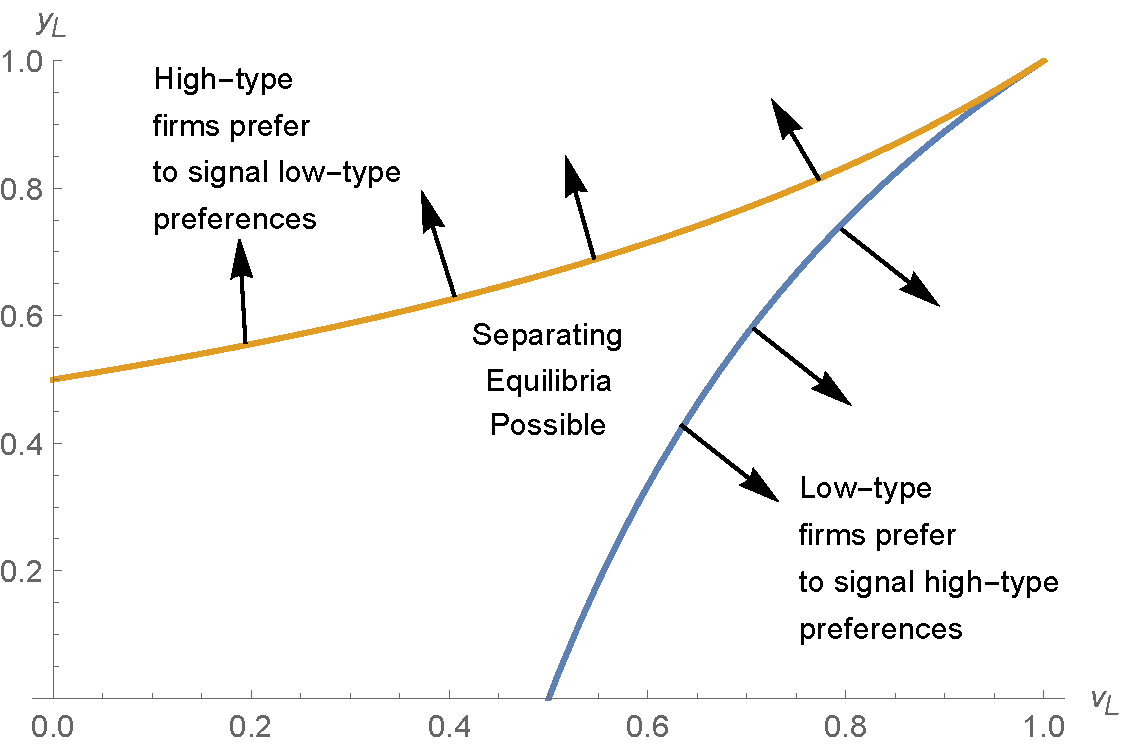
\includegraphics[width = \linewidth]{./images/illustrate_equilibria.pdf} \\
                 {\footnotesize
                   \begin{singlespace}
                     \emph{Notes:} This figure shows the possible values for low-type firms (on the x-axis) and the productivity of low-type workers (on the y-axis).
                     The two curves illustrate the indifference conditions for the two types of firms with respect to the separating equilibria. 
  \end{singlespace}
}
\end{minipage} 
\end{figure} 

\paragraph{Binary signal - sorting}
Now consider an equilibrium in which workers condition on the signal and apply to the firm that matches their type.
The firm payoffs are now
\begin{align}
  \pi_H = \frac{1}{2} \quad \mbox{and} \quad  \pi_L = \frac{1}{2} v_L y_L. \nonumber 
\end{align}
Empirically, we explore sorting both in research question (\ref{q3}), which focuses on composition, and research question (\ref{q4}), which focuses on the size of the pools. 
In this simple model, because the two sides are the same size, applicant pool are not changed.
This assumption, while clearly a simplification, seems reasonable in our setting, in that as we will show, there is little evidence of a net change in the size of applicant pools. 

When will the full separating equilibrium be obtainable?
For the high-type firm, the incentive compatibility constraint is $\frac{1}{2} \ge y_L - \frac{1}{2} v_L y_L$  whereas for the low-type firm it is $\frac{1}{2} v_L y_L \ge v_L - \frac{1}{2}$.

Figure~\ref{fig:illustrate_equilibria} illustrates how the $y_L$ and $v_L$ values affect whether a separating equilibrium is possible.
It shows the indifference curves for both types of firms.
For a high-type firm, we can see that as $y_L$ gets higher, sending the low-type signal becomes more attractive, as getting paired with a low-type worker is not as bad. 
However, as $v_L$ increases, the minimum $y_L$ for the high-type firm to switch increases, as it means low-type firms have to pay higher wages.

For a low-type firm, the higher the $v_L$, the higher the labor costs, making signaling a low-type less attractive.
Furthermore, the higher the $v_L$, the more the low-type firm values productivity, making sending the high-type signal more attractive.
With respect to workers, the lower $y_L$, i.e., the worse the workers obtained when signaling low preferences, the more attractive it becomes for a low-type firm to claim high-type preferences. 
The space between the two incentive compatibility indifference curves is the region that can support an incentive compatible separating equilibrium. 

\paragraph{Incentive compatability} 
We have so fare focused on the incentive of the firm.  
We model the firm has getting the average productivity of the pool workers, which implicitly assumes that firms cannot condition on individual productivity.  
Of course, if this were literally true, low-type workers would have strong incentive to apply to high-type employers, as this sector would pay a higher wage. And if low-type workers did this, the separating equilibrium would not be sustainable, and so firms must some ability to tell worker types apart, but not such a fine-tuned ability that they do not benefit from the separating equilibrium.

One modeling elaboration is to give high-type firms in a separating equilibrium some ability to detect a low-type worker ``sneaking in'' to the wrong market. 
Suppose a high-type firm can tell with probability $p > 0$ is they are paired with a low-productivity worker.
If the firm detects a low-productivity type, it does not make a hire.
Incentive compatibility for the low-type worker is simply that $v_L y_L > (1-p)$. 
Our research question (\ref{q3}) is whether workers condition on signals and sort to the appropriate job opening.

The surplus in a separating equilibrium in greater than pooling equilibrium if 
\begin{align}
  1 + v_L y_L > \left(\frac{1 + y_L}{2} \right) \left(\frac{1 + v_L}{2} \right),
\end{align}
which is always the case. 
Our research question (\ref{q7}) focuses changes in proxies for match surplus, such as the number of hours-worked. 
%% The surplus in the separating equilibrium is
%% \begin{align}
%%   S \propto  1 + v_L y_L 
%% \end{align}
%% whereas in the pooling equilibria, it was
%% \begin{align}
%%   S \propto \mathbb{E}[y](1 + v_L)
%% \end{align}

%% The separating equilibrium is preferable so long as $v_L < (1-\gamma)/\gamma$.
%% If $\gamma$ is very high, meaning the worker pool is mostly high, then the pooling equilibrium is attractive because a larger fraction of the work is done by high-type workers.
%% As $v_L$ gets large, the separating equilibria is less attractive because a pairing with with a low-type firm is almost as good as with a high-type firm. 
